%%%%%%%%%%%%%%%%%%%%%%%% editor.tex %%%%%%%%%%%%%%%%%%%%%%%%%%%%%
%
% sample root file for the contributions of a "contributed volume"
%
% Use this file as a template for your own input.
%
%%%%%%%%%%%%%%%%%%%%%%%%%%%%% Springer %%%%%%%%%%%%%%%%%%%%%%%%%%


% RECOMMENDED %%%%%%%%%%%%%%%%%%%%%%%%%%%%%%%%%%%%%%%%%%%%%%%%%%%
\documentclass[graybox, envcountchap, tocaftauthskip, 12pt]{svmult}
% \documentclass{simcenterdocumentation}

\usepackage{microtype}

%% use geometry to reduce the margins
\usepackage{geometry}
\geometry{
    letterpaper,
    heightrounded,
    hratio=1:1
}

%% set the reference style
\usepackage{natbib}
\bibliographystyle{abbrvnat}
\setcitestyle{authoryear,open={(},close={)}}
\setlength{\bibsep}{5pt}

% choose options for [] as required from the list
% in the Reference Guide

%\usepackage{type1cm}        % activate if the above 3 fonts are 
                             % not available on your system
                             
\usepackage{comment}

\usepackage{makeidx}         % allows index generation
\usepackage{graphicx}        % standard LaTeX graphics tool
                             % when including figure files
\usepackage{multicol}        % used for the two-column index
\usepackage[bottom]{footmisc}% places footnotes at page bottom

\usepackage{newtxtext}       % 
\usepackage{newtxmath}       % selects Times Roman as basic font

\usepackage{placeins}        % allows the use of floatbarriers
\usepackage{tabularx}        % creates tables that automatically adjust to contents
\usepackage{booktabs}        % allows the use of \midrule 
\usepackage{soul}            % highlighting

\usepackage{hyperref}
\hypersetup{
    linkcolor=blue,
}

% see the list of further useful packages in the Reference Guide

\makeindex             % used for the subject index
                       % please use the style svind.ist with
                       % your makeindex program

%%%%%%%%%%%%%%%%%%%%%%%%%%%%%%%%%%%%%%%%%%%%%%%%%%%%%%%%%%%%%%%%%

\usepackage{import}

\begin{document}

\frontmatter%%%%%%%%%%%%%%%%%%%%%%%%%%%%%%%%%%%%%%%%%%%%%%%%%%%%%%

%%%%%%%%%%%%%%%%%%%%%%%% dedic.tex %%%%%%%%%%%%%%%%%%%%%%%%%%
%
% sample dedication
%
% Use this file as a template for your own input.
%
%%%%%%%%%%%%%%%%%%%%%%%% Springer Nature%%%%%%%%%%%%%%%%%%%%%%%%%%

\begin{dedication}
Use the template \emph{dedic.tex} together with the Springer Nature document class SVMono for monograph-type books or SVMult for contributed volumes to style a quotation or a dedication\index{dedication} at the very beginning of your book
\end{dedication}




%%%%%%%%%%%%%%%%%%%%%%%foreword.tex%%%%%%%%%%%%%%%%%%%%%%%%%%%
% sample foreword
%
% Use this file as a template for your own input.
%
%%%%%%%%%%%%%%%%%%%%%%%% Springer %%%%%%%%%%%%%%%%%%%%%%%%%%

\foreword

Use the template \textit{foreword.tex} together with the document class SVMono (monograph-type books) or SVMult (edited books) to style your foreword\index{foreword}. 

The foreword covers introductory remarks preceding the text of a book that are written by a \textit{person other than the author or editor} of the book. If applicable, the foreword precedes the preface which is written by the author or editor of the book.


\vspace{\baselineskip}
\begin{flushright}\noindent
Place, month year\hfill {\it Firstname  Surname}\\
\end{flushright}



%%%%%%%%%%%%%%%%%%%%%%preface.tex%%%%%%%%%%%%%%%%%%%%%%%%%%%%%%%%%%%%%%%%%
% sample preface
%
% Use this file as a template for your own input.
%
%%%%%%%%%%%%%%%%%%%%%%%% Springer %%%%%%%%%%%%%%%%%%%%%%%%%%

\preface

This report is a product of the NSF NHERI SimCenter and provides an overview and review of simulation requirements and software tools for natural hazards engineering of the built environment. The simulations discussed in this report are an essential component of research to address the three grand challenge areas and associated research questions outlined in the NHERI Science Plan \citep{edge2020natural}. As outlined in the NHERI Science Plan, the grand challenges entail: (1) identifying and quantifying the characteristics natural hazards that are damaging to civil infrastructure and disruptive to communities; (2) evaluating the physical vulnerability of civil infrastructure and the social vulnerability of populations in at-risk communities; and (3) creation of technologies and tools to design, retrofit, and operate a resilient and sustainable infrastructure for the nation. Accordingly, required simulation technologies encompass a broad range of phenomena and considerations, from characterization and simulation of natural hazards and their damaging effects on buildings and civil infrastructure, to quantifying the resulting economic losses, disruption, and other consequences on society. Ultimately, the goal is to enable high-fidelity and high-resolution models in regional simulations that can support technological, economic, and policy solutions to mitigate the threat of natural hazards.

The natural hazards addressed in this report include earthquakes, tsunami, storm and tornado winds, and storm surge. While not an exhaustive list of all possible natural hazards, these are the hazards addressed under the U.S. National Science Foundation's (NSF) NHERI research program. The first chapter of the report provides an introduction to the SimCenter and its goals, including an overview of the plans and status for software tool development.  The subsequent chapters of the report are organized into five parts in a sequential fashion, including: (1) simulation methods to characterize the natural hazards; (2) response simulation of structural and geotechnical systems and localized wind and water flows; (3) quantifying the resulting damage and its effects on the performance of buildings, transportation systems, and utility infrastructure systems; (4) strategies and emerging tools to model recovery from natural disasters; and (5) the cross-cutting applications of uncertainty quantification methods and artificial intelligence to natural hazards engineering . 

Owing to the broad scope of the simulation topics, this state-of-art review is presented with the goal of educating and informing researchers, including both simulation tool developers and users, on key requirements and capabilities within each simulation topic. The report is also a guide for the development of simulation capabilities by the NSF NHERI SimCenter. Each chapter of the report begins with a brief overview of the purpose of the simulation component, including a discussion of the goals of the analysis (what is being calculated), the underlying physics or principles involved in the simulation, common modeling assumptions and simplifications, and typical input and output of the simulations. 

With the aim to take stock of computational simulation capabilities, inform research by the NHERI research community, and position the work of the NHERI SimCenter, the summaries identify and review commonly used simulation software that is widely known and used for research in academia and industry. Particular emphasis is placed on open-source or other software that is hosted on DesignSafe or is otherwise easily accessible to researchers, and a summary table of the simulation software tools is provided as an appendix to the report. In addition to summarizing the state-of-art in the various topic areas, each chapter of the report identifies major research gaps and needs, with the intent that these could motivate research proposals to NSF or other agencies that will lead to future advancements.

This report is an update to a state-of-the art report that the SimCenter first published in February 2019.  This update reflects comments and suggestions that were solicited from leading researchers in natural hazards engineering, and it also includes new chapters on disaster recovery modeling and applications of artificial intelligence technologies to natural hazards engineering.  Readers are encouraged to contribute feedback regarding this report and the SimCenter simulation tool development through the online SimCenter Forum at http://simcenter-messageboard.designsafe-ci.org/smf/.


\vspace{\baselineskip}
\begin{flushright}\noindent
Stanford University,\hfill {\it Gregory G. Deierlein}\\
December, 2020\hfill {\it Adam Zsarnóczay}\\
\end{flushright}



%%%%%%%%%%%%%%%%%%%%%%acknow.tex%%%%%%%%%%%%%%%%%%%%%%%%%%%%%%%%%%%%%%%%%
% sample acknowledgement chapter
%
% Use this file as a template for your own input.
%
%%%%%%%%%%%%%%%%%%%%%%%% Springer %%%%%%%%%%%%%%%%%%%%%%%%%%

\extrachap{Acknowledgements}

This material is based upon work supported by the National Science Foundation under Grant No. 1612843. Any opinions, findings, and conclusions or recommendations expressed in this material are those of the authors and do not necessarily reflect the views of the National Sci-ence Foundation or the Regents of the University of California



\setcounter{tocdepth}{1}
\tableofcontents

%%%%%%%%%%%%%%%%%%%%clist.tex %%%%%%%%%%%%%%%%%%%%%%%%
%                                                    
% sample list of contributors and their addresses    
%                                                    
% Use this file as a template for your own input.    
%                                                    
%%%%%%%%%%%%%%%%%%%%%%%% Springer %%%%%%%%%%%%%%%%%%%%
\contributors

\begin{thecontriblist}
\textbf{Pedro Arduino}
\at Professor, University of Washington
\and
\textbf{Jack W. Baker}
\at Professor, Stanford University
\and
\textbf{Jonathan D. Bray}
\at Professor, University of California, Berkeley
\and
\textbf{Henry Burton}
\at Associate Professor, University of California, Los Angeles
\and
\textbf{Luis Ceferino}
\at Assistant Professor, New York University
\and
\textbf{Barbaros Cetiner}
\at Postdoctoral Researcher, University of California, Los Angeles
\and
\textbf{Arindam G. Chowdhuri}
\at Professor, Florida International University
\and
\textbf{Joel P. Conte}
\at Professor, University of California, San Diego
\and
\textbf{Craig A. Davis}
\at TODO: ?
\and
\textbf{Gregory G. Deierlein}
\at Professor, Stanford University
\and
\textbf{George Deodatis}
\at Professor, Columbia University
\and
\textbf{Wael Elhaddad}
\at Postdoctoral Researcher, University of California, Berkeley
\and
\textbf{Ann-Margaret Esnard}
\at Professor, Georgia State University
\and
\textbf{Michael Gardner}
\at Assistant Professor, University of Nevada, Reno
\and
\textbf{Catherine Gorlé}
\at Assistant Professor, Stanford University
\and
\textbf{Sanjay Govindjee}
\at Professor, University of California, Berkeley
\and
\textbf{Sascha Hornauer}
\at Postdoctoral Researcher, University of California, Berkeley
\textbf{Liang Hu}
\at Graduate Research Assistant, University of Notre Dame
\and
\textbf{Ahsan Kareem}
\at Professor, University of Notre Dame
\and
\textbf{Tracy Kijewski-Correa}
\at Associate Professor, University of Notre Dame
\and
\textbf{Seung Jae Lee}
\at Associate Professor, Florida International University
\and
\textbf{Kincho H. Law}
\at Professor, Stanford University
\and
\textbf{Rick Luettich}
\at Professor, University of North Carolina, Chapel Hill
\and
\textbf{Patrick J. Lynett}
\at Professor, University of Southern California
\and
\textbf{Lance Manuel}
\at Professor, University of Texas, Austin
\and
\textbf{David McCallen}
\at Professor, University of Nevada, Reno
\and
\textbf{Frank McKenna}
\at Project Scientist, University of California, Berkeley
\and
\textbf{Yuki Miura}
\at Graduate Research Assistant, Columbia University
\and
\textbf{Michael Motley}
\at Associate Professor, University of Washington
\and
\textbf{Thomas O'Rourke}
\at Professor, Cornell University
\and
\textbf{Satish Rao}
\at Professor, University of California, Berkeley
\and
\textbf{Paneer Selvam}
\at Professor, University of Arkansas
\and
\textbf{Michael D. Shields}
\at Associate Professor, Johns Hopkins University
\and
\textbf{Rodrigo Silva-Lopez}
\at Graduate Student, Stanford University
\and
\textbf{Vesna Terzic}
\at Associate Professor, California State University, Long Beach
\and
\textbf{Ertugrul Taciroglu}
\at Professor, University of California, Los Angeles
\and
\textbf{Alexandros Taflanidis}
\at Associate Professor, University of Notre Dame
\and
\textbf{Iris Tien}
\at Associate Professor, Georgia Institute of Technology
\and
\textbf{Chaofeng Wang}
\at Postdoctoral Researcher, University of California, Berkeley
\and
\textbf{Qian Yu}
\at Postdoctoral Researcher, University of California, Berkeley
\and
\textbf{Stella Yu}
\at Director, Vision Group, ICSI, University of California, Berkeley
\and
\textbf{Adam Zsarnóczay}
\at Postdoctoral Researcher, Stanford University 
\end{thecontriblist}
%%%%%%%%%%%%%%%%%%%%%%acronym.tex%%%%%%%%%%%%%%%%%%%%%%%%%%%%%%%%%%%%%%%%%
% sample list of acronyms
%
% Use this file as a template for your own input.
%
%%%%%%%%%%%%%%%%%%%%%%%% Springer Nature%%%%%%%%%%%%%%%%%%%%%%%%%%

\extrachap{Acronyms}

\begin{description}[CABR]

\item[AI]{Artificial Intelligence}
\item[CFD]{Computational Fluid Dynamics}
\item[CGS]{California Geological Survey}
\item[CS]{Conditional Spectrum}
\item[DM]{Damage Measure}
\item[DNS]{Direct Numerical Simulation}
\item[DRM]{Dimension Reduction Methods}
\item[DV]{Decision Variable}
\item[FEMA]{Federal Emergency Management Agency}
\item[GMM]{Ground Motion Model}
\item[GMPE]{Ground Motion Prediction Equation}
\item[GMR]{Ground Motion Record}
\item[HPC]{High-Performance Computing}
\item[IBM]{Immersed Boundary Method}
\item[IM]{Intensity Measure}
\item[IT]{Information Technology}
\item[LBM]{Lattice Boltzmann Method}
\item[LES]{Large Eddy Simulation}
\item[ML]{Machine Learning}
\item[NSF]{National Science Foundation}
\item[NHE]{Natural Hazards Engineering}
\item[NHERI]{Natural Hazards Engineering Research Infrastructure}
\item[NS]{Navier-Stokes equations}
\item[PGA]{Peak Ground Acceleration}
\item[PGV]{Peak Ground Velocity}
\item[PSHA]{Probabilistic Seismic Hazard Assessment}
\item[RANS]{Reynolds-Averaged Navier-Stokes equations}
\item[Sa(T)]{Spectral Acceleration at a given T vibration period}
\item[SCEC]{Southern California Earthquake Center}
\item[SPH]{Smooth Particle Hydrodynamics}
\item[UHS]{Uniform Hazard Spectrum}
\item[USGS]{United States Geological Survey}

\end{description}

\mainmatter%%%%%%%%%%%%%%%%%%%%%%%%%%%%%%%%%%%%%%%%%%%%%%%%%%%%%%%

%%%%%%%%%%%%%%%%%%%% author.tex %%%%%%%%%%%%%%%%%%%%%%%%%%%%%%%%%%%
%
% sample root file for your "contribution" to a contributed volume
%
% Use this file as a template for your own input.
%
%%%%%%%%%%%%%%%% Springer %%%%%%%%%%%%%%%%%%%%%%%%%%%%%%%%%%%%%%%%%

\title{Introduction and SimCenter Goals}
% Use \titlerunning{Short Title} for an abbreviated version of
% your contribution title if the original one is too long
\author{
    \textbf{Sanjay Govindjee}
    \and Gregory G. Deierlein
    \and Frank McKenna}
\tocauthor{}
\authorrunning{Govindjee et al.}
% Use \authorrunning{Short Title} for an abbreviated version of
% your contribution title if the original one is too long
%\institute{Name of First Author \at Name, Address of Institute, %\email{name@email.address}
%\and Name of Second Author \at Name, Address of Institute %\email{name@email.address}}
%
% Use the package "url.sty" to avoid
% problems with special characters
% used in your e-mail or web address
%
\maketitle

Computational simulation is as an essential component of natural hazards engineering research and practice to assess and mitigate the damaging effects of earthquakes, wind storms and associated tsunami, and storm surge effects on communities. Recognizing the challenge as broad and multi-disciplinary, and encompassing natural hazards across a wide range of scales, the SimCenter's approach is to leverage existing software platforms by creating computational workflow technologies that can seamlessly integrate a broad array of simulation software with high-performance computing platforms and data repositories. In addition to developing and releasing the computational workflow tools and training modules, the SimCenter is engaging with researchers to extend the simulation capabilities through collaboration with NHERI researchers. Collaboration opportunities range from facilitating research on application testbed studies to implementation of new computational formulations.

The SimCenter is creating workflow tools that range from ones that enable the study of the response of single buildings given a natural hazard event to others that perform end-to-end simulations of natural hazard effects on communities. An important emphasis of the workflows are capabilities to incorporate and propagate inherent variabilities and modeling uncertainties through the computational simulations. Another focus is on tools to develop datasets and integrate them with the computational tools, with particular emphasis on data and simulation software available on the NHERI DesignSafe platform.

To a large extent, the most distinguishing innovation of the SimCenter simulation tools are to provide a computational ecosystem that will enable the NHERI research community to achieve unprecedented capabilities to conduct end-to-end simulations. By employing an open-source framework, the ecosystem will allow researchers to contribute to some or all aspects of the simulation capabilities. The overall concept is illustrated in Figure \ref{fig:intro_CompFramework}, where the challenge is to link models and data from descriptions of the assets (buildings, bridges, civil infrastructure, and other components of the built environment), hazard effects (earthquake ground motions, wind, water inundation), through to effects on the assets and implications on community function and recovery. The SimCenter computational and data tools lie at the heart of the simulation, linking upstream data from natural hazard models to downstream socio-economic outcomes and models of communities. Figure \ref{fig:intro_CompFramework} illustrates where four SimCenter tools (uqFEM, EE-UQ, CWE-UQ, and PBE) fit into the computational workflow. Underlying these tools are software applications that can be incorporated in specific tools (with graphical user interfaces) or incorporated in workflow scripts that are more fluid and adaptable to alternative regional hazard scenario simulations. 

\begin{figure}[htb]
    \centering
    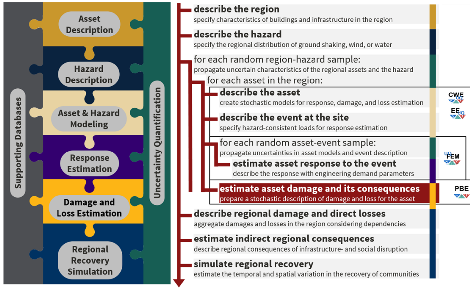
\includegraphics[width=1.0\textwidth, angle = 0]{editor/Figures/CompFramework.pdf}
    \caption{Computational framework for end-to-end simulations of natural hazard effects on damage and recovery of the built environment and communities}
    \label{fig:intro_CompFramework}
\end{figure}

The following is a summary of computational workflow implementations that the SimCenter is actively working on and has either already deployed or will deploy in the immediate future:

\paragraph{uqFEM} The uqFEM application facilitates uncertainty quantification, model calibration, optimization and sensitivity analyses of structural and geotechnical materials, components, and systems by combining existing finite element applications with uncertainty quantification (UQ) application. The V1.1.0 release links two finite-element codes (OpenSEES or FEAPpv) with uncertainty quantification functions in DAKOTA. A graphical user interface is provided with basic functionality to define random variables in the finite-element models and invoke certain UQ methods from DAKOTA. Running through the HPC capabilities of DesignSafe, or on a user's desktop computer, the system makes available unprecedented capabilities for natural hazards researchers to perform UQ simulations. Future plans include extensions to include links to other finite element codes that are running on DesignSafe (e.g., LSDyna) and uncertainty quantification toolboxes (UQ-Pyt, UQpy).
%\newline

\paragraph{CWE-UQ} The Computational Wind Engineering (CWE) Tool is an application to simulate the response of structures to wind forces. The V2.0 release of the tool will allow users to select from a variety of options for specifying wind forces on structures from stochastic loading models and online wind engineering databases through to performing computationally intense Computational Fluid Dynamics (CFD) analysis utilizing applications such as OpenFOAM. The tool is intended to make detailed CFD modeling more accessible to NEHRI researchers in conjunction with wind tunnel testing (e.g., to validate computational models and extrapolate beyond the scale and parameter space that can be tested in the NHERI wind facilities), to allow researchers to consider more realistic conditions from field studies, and assist in the creation of surrogate models for regional simulations. For the CFD analysis in particular, the CWE-UQ tool is organized around a template-based model. Currently (in V1.1.1) there are two templates: 2D simulation of a rigid building geometry using an unstructured mesh; and 3D simulation of a rigid building using an unstructured mesh. Capabilities for the simulation of desired inflow conditions for LES, aeroelastic response, and multi-fidelity simulations are in the development stage. 
Exploratory work is underway to investigate adaptation of the CWE-UQ tool to simulate water flows for modeling tsunami or storm surge effects on structures. Future releases will incorporate Uncertainty Quantification (UQ) in a similar fashion to uqFEM.
%\newline

\paragraph{EE-UQ} The earthquake engineering, EE-UQ, tool is an application to simulate the response of structural and soil–structure systems to earthquake excitations. The current (V1.0) release focuses on quantifying the uncertainties in the structural response, given that the properties of buildings (or other structures) and the earthquake events are not known exactly, and that many simplifying assumptions are present in the numerical models (epistemic uncertainties). By embedding features of the uqFEM tool, EE-UQ enables the user to specify statistical distributions of the model input parameters and Monte Carlo and other sampling methods are used to characterize the output. The current implementation employs OpenSees for finite-element simulation of the structural models and DAKOTA for uncertainty propagation. The tool has features to select and input ground motions to match specified earthquake hazard targets. Work is underway to extend EE-UQ to include soil-structure interaction models where rock ground motions are propagated through nonlinear soil models into the structural system.
%\newline

\paragraph{PBE} The PBE tool is an extensible workflow application to perform Performance Based Engineering computations for various hazards. The current (V1.0) release provides researchers a tool to assess the performance of a building subjected to earthquake ground motions. The application focuses on quantifying nonlinear building response and damage through decision variables. PBE builds upon the EE-UQ tool using the estimates of structural response to assess the damage to building components and the consequences of such damage. The user characterizes the simulation model, and the damage and loss models of the structure, and the seismic hazard model in the PBE tool. The tool incorporates an underlying workflow application called PELICUN (Probabilistic Estimation of Losses, Injuries, and Community resilience Under Natural disasters), which is a hazard and asset agnostic library for evaluating losses. PELICUN is modeled after the FEMA P58 framework for earthquake loss assessment but with a broader vision to address alternate hazards (wind, water inundation, etc.) and facilities beyond buildings. All components within the PBE tool are interconnected by an uncertainty quantification framework that allows the user to define a flexible stochastic model for the problem.
%\newline

\paragraph{RDT} The RDT tool is to be an extensible workflow application to quantify the effects of hazards on regional communities. This tool is scheduled for initial release in 2020. It will provide the users with options for selecting regions, hazards, and viewing the results at a regional scale. The tool will utilize much of the workflow developed for the CWE-UQ, EE-UQ, and PBE tools. As part of the development of the tool, two command line workflow applications are being developed and made available: (1) the Regional Earthquake Workflow and (2) the Regional Storm Workflow. The RDT tool, when completed, will provide a graphic front-end to these command line applications.
%\newline

\paragraph{Regional Earthquake Workflow} The Regional Earthquake Workflow is an application to quantify the damaging effects of earthquakes on society at a regional scale. The workflow implements a comprehensive end-to-end hazard simulation along the lines shown in Figure \ref{fig:intro_CompFramework}. Further details of the workflow, including definitions of the workflow components, are shown in Figure \ref{fig:intro_CompWorkflow}. Two testbed examples have been released to demonstrate the Regional Earthquake Workflow. The first testbed estimates downtime and loss for every building in the San Francisco Bay Area after a simulated magnitude 7.0 earthquake on the Hayward fault. The second testbed is a smaller study on the 2018 M7.0 event in Anchorage, Alaska. Following a similar strategy to the other SimCenter tools, the workflow integrates various stand-alone software applications and modules. Some applications, such as “performSIM”, utilize existing software such as OpenSees, whereas other applications are developed specifically for the initial testbed workflow. Two instances of the framework application were developed: (1) HPC resources at DesignSafe are used for simulation of a large (1.6 million) inventory of buildings, and (2) local computational resources for testing, development, and smaller-scale simulations (thousands of buildings) are used. The workflow applications are seeded with ground-motion tools and data sets to show extensibility and provide resources that inspire research activities. In the coming year, a Regional Storm Workflow is being developed, that will parallel the earthquake scenario testbed for a hurricane scenario testbed at a location on the eastern coast of New Jersey.

\begin{figure}[htb]
    \centering
    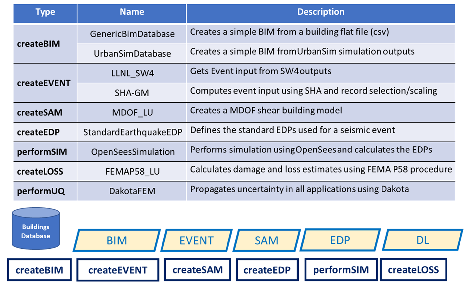
\includegraphics[width=1.0\textwidth, angle = 0]{editor/Figures/CompWorkflow.pdf}
    \caption{Computational workflow and registered applications for the San Francisco Bay Area Earthquake Scenario}
    \label{fig:intro_CompWorkflow}
\end{figure}

\paragraph{AI Applications} One of the key challenges for building regional hazard scenarios is creation of actual BIMs (Building Information Models) and SAMs (Structural Analysis Models) for the buildings in the region. To address this, the SimCenter has ongoing development to apply Artificial Intelligence (AI) methods to develop ``aiBIM'' and ``aiSAM'' applications. The ``aiBIM'' application utilizes visual imagery combined with other databases (e.g., parcel level tax data, LIDAR imagery, etc.) to develop a detailed database of buildings and their features. The ``aiSAM'' application translates BIM information into SAM to simulate the damaging effects of earthquakes, wind, and water inundation.
%\newline

\noindent This report has laid out the state of the art as seen by the authors of the respective sections as of the date of this report and how the SimCenter's current and future developments are aligned with these observations. The report thus serves not only as a state-of-the-art report for general consumption but also as a guiding document for the SimCenter. We hope that its contents find wide use and help focus research and software development needs in the NHERI community.



\begin{partbacktext}
\part{Hazard Characterization}
\label{part:hazard}

Characterization of natural hazards for engineering applications aims to quantify the severity of a natural hazard at a particular location or over a pre-defined region of interest. The time histories that provide a detailed description of natural-hazard effects such as ground shaking or high-speed winds are often summarized by so-called Intensity Measures (IMs) that represent their most important characteristics. Peak ground acceleration, permanent ground deformation, average one-minute wind speed, and peak inundation depth are a few examples of such IMs for various natural hazards. The limited number of parameters facilitates the development of a stochastic hazard model that defines the hazard severity at the site(s) of interest using one more more random variables or random fields. The uncertainty in the hazard that is captured by these random entities shall be propagated through the engineering simulation. 

High-fidelity approaches simulate the response of the built environment using dynamic, response-history analyses (see Part \ref{part:response} for details). These simulations require a time-dependent load function that shall represent the hazard characterized by the IMs. An acceleration time history of a ground motion is an example of such a load function, which is often used for seismic response estimation. These load functions are either selected from historical data (e.g., ground-motion records) or generated using a stochastic process (e.g., local wind inflow conditions for a CFD simulation). The procedures and best practices available for this task will be discussed for each natural hazard below.

Three types of natural hazards are examined in the following sections: earthquake, hurricane, and tsunami. They present several fundamentally different threats to the built environment, such as ground shaking and liquefaction under earthquakes, or wind and storm surge under hurricanes. Each chapter in this part discusses one of those threats to the built environment.

\end{partbacktext}
\import{Hazard/Earthquake_Ground_Shaking/}{main}
\import{Hazard/Earthquake_Surface_Rupture/}{main}
\import{Hazard/Earthquake_Liquefaction/}{main}
\import{Hazard/Earthquake_Landslide/}{main}
\import{Hazard/Storm_Wind/}{main}
\import{Hazard/Storm_Surge/}{main}
\import{Hazard/Tsunami/}{main}


\begin{partbacktext}
\part{Response Estimation}
\label{part:response}

Response estimation entails computational finite-element and other analysis methods to simulate the physical response of solids and fluids related to natural hazards engineering. The section on structural systems describes simulation technologies to analyze the response of constructed facilities (buildings, bridges, and other facilities) to the loading effects of gravity, earthquakes, storms (wind and storm-surge flows), and tsunami inundation. The section on geotechnical systems describes methods to explicitly simulate the detailed response of soil and soil–structure interaction under input ground motions. The simulation results are used to determine ground deformations, liquefaction, soil–structure interaction, and ground instabilities due to other phenomena (e.g., changes in ground water levels, scour, etc.). The sections on computational fluid dynamics address methods to simulate wind and water flows due to water inundation and tsunami. 

\end{partbacktext}
\import{Response/Structural/}{main}
\import{Response/Geotechnical/}{main}
\import{Response/CFD_Wind/}{main}
\import{Response/CFD_Water/}{main}


\begin{partbacktext}
\part{Performance Assessment}\label{part:Performance}

The built environment is a collection of various types of assets that affect the well-being and quality of life of residents in an urban area. The list of such assets includes residential and commercial buildings, bridges, networks of roads, railways, pipelines and power lines, and their supporting facilities. The performance of these assets is quantified by Decision Variables (DV) that describe the influence of asset damage to the life of the affected community. As their name implies, these DVs are ultimately meant to drive decision- and policy-making.

The performance of assets heavily depends on the determination of the hazard and the asset response to a characteristic event that is consistent with the hazard at the asset location. Although this chapter focuses on performance assessment, some of the tools listed here have hazard and response estimation capabilities as well. Those features have been covered in the previous chapters and will not be mentioned here again. This chapter is organized around the types of assets or asset-networks needed to arrive at a description of the performance of an urban region. 

Seismic performance assessment of buildings has received a lot of attention from the research community and funding agencies in the past few decades (ATC, 1985; FEMA Mitigation Division, 2018b, 2018c; Fajfar and Krawinkler, 2004; FEMA, 2012). Consequently, the most sophisticated and mature methods are available in that area (FEMA, 2012). Several researchers have focused on adopting these methods for other asset types (werner2006redars; chmielewski2016response) and for other types of hazards (FEMA Mitigation Division, 2018c; attary2017performancebased; barbato2013performancebased; lange2014application). This is not a trivial task because damage and subsequent consequences can be fundamentally different for non-building assets and for non-seismic disasters.  

\end{partbacktext}

\import{Performance/Buildings/}{main}
\import{Performance/Transportation/}{main}
\import{Performance/Pipelines/}{main}
\import{Performance/Power/}{main}


\begin{partbacktext}
\part{Recovery Modeling}

This section provides an introductory discussion on the modeling of disaster recovery for infrastructure, residential buildings, businesses, and communities. The aim of this section is not to present an exhaustive list or propose an ideal approach given the complexity of the recovery process and the wide variation across hazard types and geographies. Empirical studies are reviewed to identify factors that are associated with recovery, providing the basis for conceptual models of recovery. It is also noted that, although, recovery simulations are often used to obtain proxies of the disaster resilience, disaster recovery is only one among many metrics of resilience \citep{national2019building,kwasinski2016conceptual}. For this reason, the scope of this section does not include a comprehensive review of the broader topic of disaster resilience.\

Disaster recovery modeling consists of assessing over time the performance of a system subjected to a shock. Prior to the shock, the system has a baseline state, $Q_b$. At the time of the event, $t_0$, disturbances to the system reduce its functionality to a new state, $Q_0$. Subsequently, the system is restored until a time $t_R$ when its new normal is established. Recovery may be partial, with the new normal below the pre-disaster state. Or, improvements may be done to the system and the new normal is an improvement. While comparing recovery with pre-disaster state is a common practice, another alternative is to compare it to the projected state of the system had the shock not occurred. Plotting the state of the system over time, $Q(t)$, against the time since the shock provides a graph as the one shown in Figure \ref{fig:ResilienceTriangle}. The curve $Q(t)$ is called the recovery trajectory \citep{Bruneau2003}. While loss assessments focus on the magnitude of the initial drop in the functionality of the system, recovery modeling is devoted to simulating the recovery trajectory. Hence, the main output from a recovery model is the time series of $Q(t)$.\

\begin{figure}[htb]
    \centering
    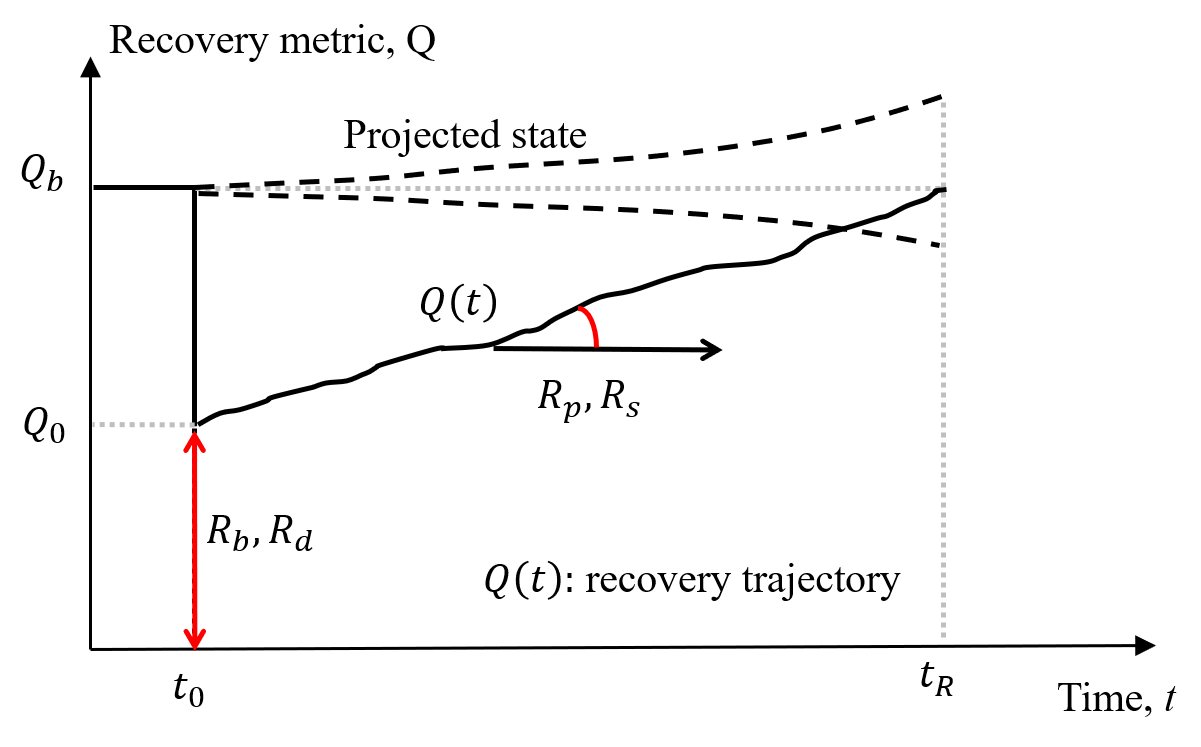
\includegraphics[width=0.7\textwidth, angle = 0]{Resilience_Concepts.png}
    \caption{Resilience triangle. Adapted from \cite{Bruneau2003}.}
    \label{fig:ResilienceTriangle}
\end{figure}

The magnitude of the initial drop at $t_0$ is a function of the robustness, $R_b$, and the redundancy, $R_d$, of the system. A perfectly robust system is one that can experience a shock without significant changes. A perfectly redundant system is one that, if disrupted, can immediately and cost effectively rearrange itself to provide the same level of service as before the event. The ability of the system to regain functionality can be estimated from the slope of the recovery trajectory. The slope is influenced by the capacity of the system to mobilize resources and meet priorities. These are often called the system's resourcefulness, $R_s$, and rapidity, $R_p$ \citep{Bruneau2003}. The concepts in Figure \ref{fig:ResilienceTriangle} can be employed to study the recovery of critical infrastructure, housing, and businesses. The following sections discuss the state of the art in simulation the recovery of these three systems.\

\FloatBarrier
\end{partbacktext}
\import{Recovery/Communities/}{main}
\import{Recovery/Infrastructure_Systems/}{main}
\import{Recovery/Housing/}{main}
\import{Recovery/Businesses/}{main}


\begin{partbacktext}
\part{Cross-cutting methodologies}
\label{part:cross}

This section of the report examines two related cross-cutting topics, uncertainty quantification and artificial intelligence, which have applications across all phases of natural hazards engineering (NHE).  Both areas are developing rapidly, propelled by the capabilities of modern high-performance computing (HPC), information technologies (IT), and data harvesting technologies, and supported by algorithmic developments.  

Uncertainty Quantification (UQ) covers a broad range of topics that include (1) characterization of uncertainties in natural hazards, their damaging effects on the built environment, and the resulting consequences on communities, (2) propagation of uncertainties through simulations of natural hazards through to their consequences, (3) statistical calibration of simulation models, including Bayesian inference methods to update models with observed data, and (4) design under uncertainty, including design of physical assets through to strategies and practices to mitigate risk and promote recovery from natural disasters.  

Artificial intelligence (AI) and machine learning (ML) have a range of potential applications to NHE, the capabilities of which are just beginning to be realized.   AI/ML can be applied to (1) develop features of buildings and other assets that form the basis for simulating the effects of natural hazards on communities, (2) develop surrogate data-driven models at various scales, ranging from material models in finite element simulations, to models of natural hazard intensity parameters, to simplified models of buildings and other assets in regional simulations, and (3) detect and assimilate observational data from post-disaster reconnaissance.  As described in Chapter \ref{chapter:cc_aiml}, AI/ML tools encompass a range of techniques, including knowledge-based expert systems, statistical-based neural networks, kernel-based methods, and deep learning approaches.   While the AI/ML show great potential and promise to revolutionize NHE, success in this regard hinges on identifying appropriate uses of the technologies and taking care to validate and develop confidence in the methods.


\end{partbacktext}
\import{CrossCutting/Uncertainty/}{main}
\import{CrossCutting/AI/}{main}

%

\backmatter%%%%%%%%%%%%%%%%%%%%%%%%%%%%%%%%%%%%%%%%%%%%%%%%%%%%%%%

\begin{partbacktext}
\part{Appendix}

\appendix
%%%%%%%%%%%%%%%%%%%%% appendix.tex %%%%%%%%%%%%%%%%%%%%%%%%%%%%%%%%%
%
% sample appendix
%
% Use this file as a template for your own input.
%
%%%%%%%%%%%%%%%%%%%%%%%% Springer-Verlag %%%%%%%%%%%%%%%%%%%%%%%%%%

\chapter{List of Software Tools}
\label{tools_list} % Always give a unique label
% use \chaptermark{}
% to alter or adjust the chapter heading in the running head

Intro

\section{Hazard Characterization}
\label{sec:tools_list_hazard}
% Always give a unique label
% and use \ref{<label>} for cross-references
% and \cite{<label>} for bibliographic references
% use \sectionmark{}
% to alter or adjust the section heading in the running head
Table

\section{Response Estimation}
\label{sec:tools_list_response}

Table

\section{Performance of the Built Environment}
\label{sec:tools_list_performance}

Table

\section{Recovery Simulation}

%% Here is the information but I am not sure what is the formatting for the table
%% so I am leaving it in this placeholder style
\label{sec:tools_list_recovery}
\begin{table}[]
    \centering
    \begin{tabular}{l|cccc}
    \toprule
    Name & Categories & Public Access & Operating system & DesignSafe \\
    DESaster & All assets & OSS & All & N \\
    InCORE & All assets & OSS & All & N \\
    RecovUS & Housing & OSS & All & N \\
    Rts & All assets & OSS & W & N \\
    \bottomrule
    \end{tabular}
    \caption{Caption}
    \label{tab:my_label}
\end{table}

\noindent Public access\\
OSS: open-source software\\

\noindent Operating System:\\
W: Windows

\noindent DesignSafe\\
N: not compatible\\
Y: compatible



\section{Uncertainty Quantification}
\label{sec:tools_list_uq}

Table

\section{Artificial Intelligence and Machine Learning}
\label{sec:tools_list_ai}


\end{partbacktext}

%%%%%%%%%%%%%%%%%%%%%%acronym.tex%%%%%%%%%%%%%%%%%%%%%%%%%%%%%%%%%%%%%%%%%
% sample list of acronyms
%
% Use this file as a template for your own input.
%
%%%%%%%%%%%%%%%%%%%%%%%% Springer Nature%%%%%%%%%%%%%%%%%%%%%%%%%%

\Extrachap{Glossary}


Use the template \emph{glossary.tex} together with the Springer Nature document class SVMono (monograph-type books) or SVMult (edited books) to style your glossary\index{glossary} in the Springer Nature layout.


\runinhead{glossary term} Write here the description of the glossary term. Write here the description of the glossary term. Write here the description of the glossary term.

\runinhead{glossary term} Write here the description of the glossary term. Write here the description of the glossary term. Write here the description of the glossary term.

\runinhead{glossary term} Write here the description of the glossary term. Write here the description of the glossary term. Write here the description of the glossary term.

\runinhead{glossary term} Write here the description of the glossary term. Write here the description of the glossary term. Write here the description of the glossary term.

\runinhead{glossary term} Write here the description of the glossary term. Write here the description of the glossary term. Write here the description of the glossary term.

\bibliographystyle{abbrvnat}
\bibliography{
    zotero-refs.bib,
    % autobib-NO-EDITS,
    % Hazard/Earthquake_Surface_Rupture/references,
    % Hazard/Earthquake_Liquefaction/references,
    % Hazard/Earthquake_Landslide/references,
    % Hazard/Storm_Surge/references,
    % Response/Geotechnical/references,
    % Recovery/references,
    % references
}

\printindex

%%%%%%%%%%%%%%%%%%%%%%%%%%%%%%%%%%%%%%%%%%%%%%%%%%%%%%%%%%%%%%%%%%%%%%

\end{document}

